\documentclass{ctexart}
\usepackage[hmargin=1.1in,vmargin=1in]{geometry}
\usepackage{amsmath}
\usepackage{graphicx}
\usepackage[defaultmono]{droidsansmono}

\title{《信号处理导论》课程报告三}
\input{personal_info/info.tex}

\begin{document}
    \maketitle

    \section{我学到了哪个知识点?}

    卷积积分。卷积积分是一种对两个非离散函数进行的操作,结果为一个函数。具体来说其定义式如下:

    \[
        h(t) = (f*g)(t) = \int_{-\infty}^{+\infty} f(\tau) \cdot g(t - \tau) \mathrm{d}\tau
    \]

    也可以直观理解为将 $g(\tau)$ 的图像沿 $y$ 轴镜像之后再向 $\tau$ 轴正向移动 $t$ 单位,所得的新函数再与
    $f(\tau)$ 相乘再在 $(-\infty, +\infty)$ 上求积分所得。

    来源:《信号与线性系统分析》第四版——吴大正 2.3 节 卷积积分。

    \section{我之前是怎么想的?}

    之前在信息竞赛的学习中听到过``卷积''甚至是``狄里克雷卷积''之类的词语,但是没有深入了解它们的含义。也听说过
    ``卷积神经网络''之类的说法,大概猜想``卷积''是某些函数的乘积之类的东西,并不知道它的定义。

    \section{我之前的想法怎么样?}

    之前我对``卷积''一无所知。不过倒是已经了解了针对函数的运算(``算子''),也知道了某些利用积分来定义的针对函
    数的算子(比如说高阶函数的定义)。

    \section{我应该怎样想才对?}

    卷积是对一种特殊积分操作的称呼,并且有直观的图形化的理解与求解方法。卷积的存在同时也再一次印证了``能写出表达
    式的函数不一定是初等函数'',因为用卷积积分定义的函数其定义式已经出现了(反常)积分运算,而这种运算不属于初等
    函数的范畴。事实上卷积积分有着不少好用的性质,比如说交换律、结合律、分配率,以及积分、导数运算律等等,可以用
    来方便一些计算。

    \section{我应该怎样用上它?}

    如定义``卷积''运算那般,将常用而重要的操作、步骤、表达式等单独定义出来,并研究其性质,这是一种很常见的方法,
    比如物理学中就定义有速度 $\vec{v} = \frac{\mathrm{d}\vec{x}}{\mathrm{d}t}$、加速度
    $\vec{a} = \frac{\mathrm{d}\vec{v}}{\mathrm{d}t}$,以及程序设计上``重复的代码段尽量定义为函数''等。
    应该多学习这种思想的运用,来减少重复工作,并使得数学运算、程序编写等更加简洁、有条理。

    \section*{字数统计}

    \begin{center}
        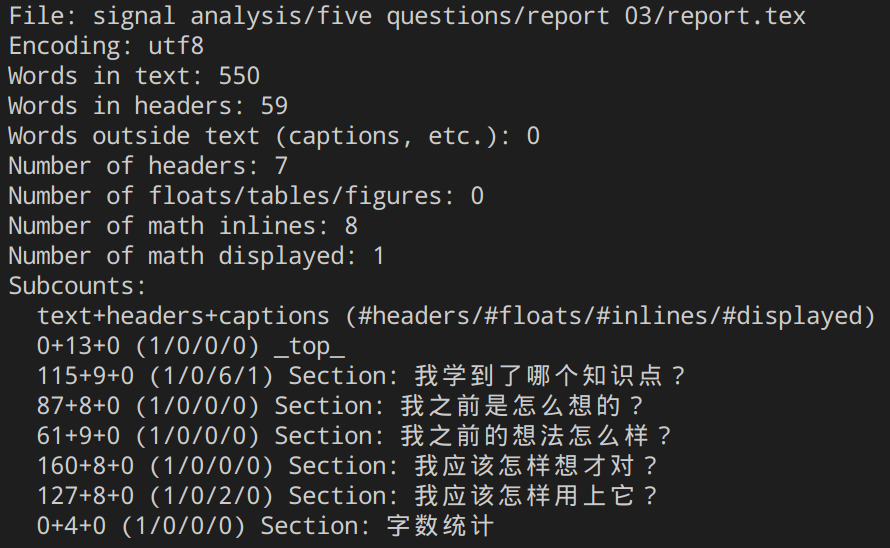
\includegraphics[width=0.8\textwidth]{pics/texcount.png}
    \end{center}
\end{document}